% Sample LaTeX file for creating a paper in the Morgan Kaufmannn two
% column, 8 1/2 by 11 inch proceedings format.

\documentclass[letterpaper]{article}
\usepackage{uai2019}
\usepackage[margin=1in]{geometry}
\usepackage{graphicx}
\usepackage{amsmath}

% Set the typeface to Times Roman
\usepackage{times}

\newcommand{\norm}[1]{\left\lVert#1\right\rVert}

\title{Denoising Graph Neural Networks}

\author{} % LEAVE BLANK FOR ORIGINAL SUBMISSION.
          % UAI  reviewing is double-blind.

% The author names and affiliations should appear only in the accepted paper.
%
%\author{ {\bf Harry Q.~Bovik\thanks{Footnote for author to give an
%alternate address.}} \\
%Computer Science Dept. \\
%Cranberry University\\
%Pittsburgh, PA 15213 \\
%\And
%{\bf Coauthor}  \\
%Affiliation          \\
%Address \\
%\And
%{\bf Coauthor}   \\
%Affiliation \\
%Address    \\
%(if needed)\\
%}

\begin{document}

\maketitle

\begin{abstract}

We present a noise-tolerrant approach to train Graph Neural Networks (GNNs) for
the graph classification task. By combining the nonlinear neural message-passing 
models (e.g. Graph Isomorphism Networks, GraphSAGE, etc.) with uncertainty 
discount procedure, we study the robustness to symmetric label noise of GNNs 
training procedures. We prove that such class of estimator on graph can adapt 
well to label noise under the untertainty discount framework. Moreover, we 
empirically demonstrate the effectiveness of our proposed training procedure. 
Our experiments show that test accuracy and generalization gap can be improved 
greatly under noisy settings. 

\end{abstract}

\section{Introduction}

\begin{figure}
  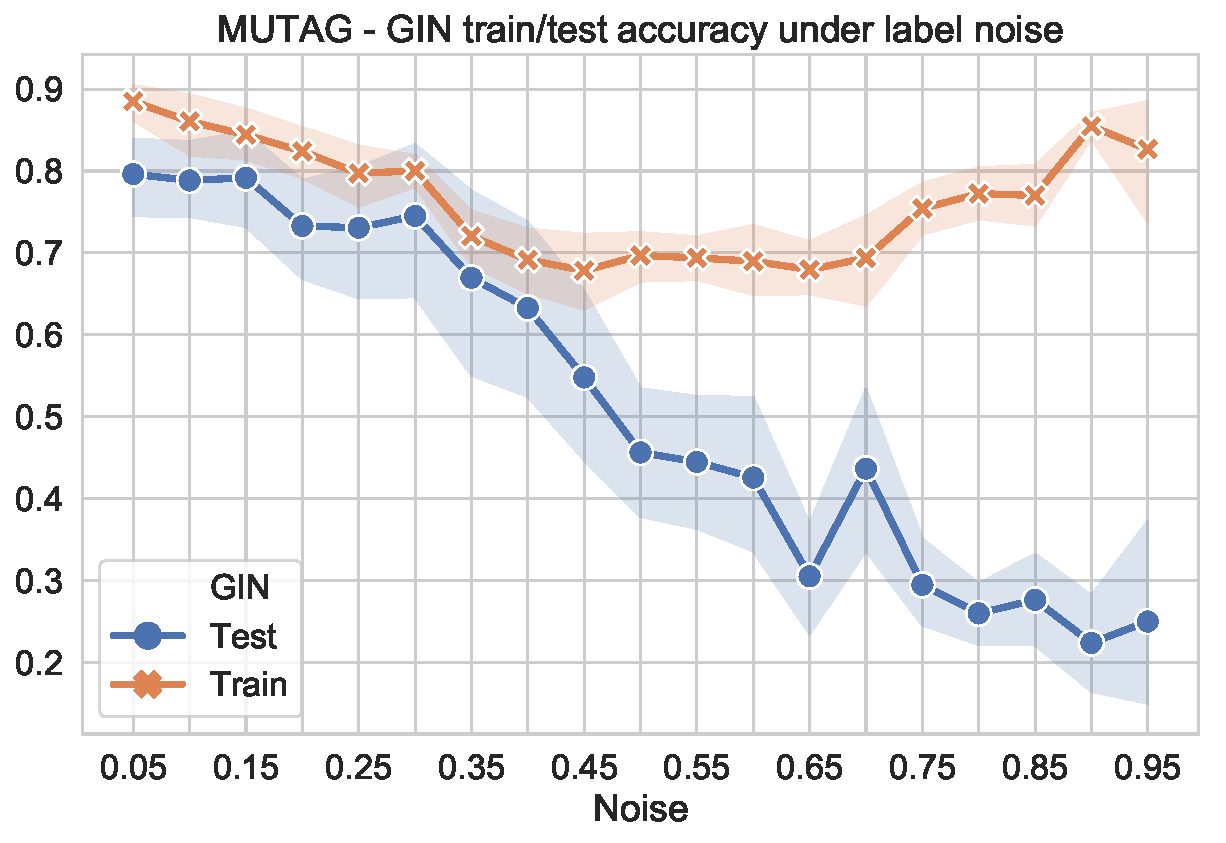
\includegraphics[width=0.5\textwidth]{figs/MUTAG_noisy_training}
  \caption{GIN model trained with increasing symmetric label noise. 
  For each label noise configuration, we train the model 10 times and 
  report the mean and standard deviation of accuracy results on the test dataset.}
  \label{fig:mutag_gin}
\end{figure}

\section{Method}

HOW ABOUT A COMBINATION OF BOTH FORWARD AND BACKWARD? 
such method doesn't seem to work.

\section{Empirical Results}

We test our framework on the set of well-studied 9 datasets for the graph 
classification task : 4 bioloinformatics datasets (MUTAG, PTC, NCI1, PROTEINS),
and 5 social network datasets (COLLAB, IMDB-BINARY, IMDB-MULTI, REDDIT-BINARY, REDDIT-MULTI5K)
\cite{gin,graphsage,anonwalk,yanardag2015}. We follow the preprocessing suggested by \cite{gin} 
to use onehot encoding as node degrees for social networks (except REDDIT datasets). 
Table \ref{t:data} gives the overview of each dataset. Since these datasets have exact 
label for each graph, we introduce symmetric label noise artificially.

\begin{table}[h]
\caption{Data overview. (*) indicates datasets having associated 
feature vector for each node.}
\label{t:data}
\begin{center}
\begin{tabular}{l|cccc}
\bf Dataset & \# graphs & \# classes & Avg. \# nodes \\
\hline \\
IMDB-B   & 1000 & 2 & 19.8  \\   
IMDB-M   & 1500 & 3 & 13.0  \\ 
RDT-B    & 2000 & 2 & 429.6 \\    
RDT-M5K  & 5000 & 5 & 508.5 \\       
COLLAB   & 5000 & 3 & 74.5  \\     
MUTAG*   & 188  & 2 & 17.9  \\    
PROTEINS*& 1113 & 2 & 39.1  \\       
PTC*     & 344  & 2 & 25.5  \\  
NCI1*    & 4110 & 2 & 29.8  \\   
\end{tabular}
\end{center}
\end{table}

\subsection{Noise Estimation}

\paragraph{Label Noise} For each datasets in Table \ref{t:data}, we corrupt
their labels with rate $n$ during training. In this research, we study the
\emph{symmetric} noise setting where label $i$ is corrupted to label $j$ 
with the same probability for $j$ to $i$ ($n_{i,j} = n_{j,i}$). We use a
$m$ by $m$ symmetric Markov matrix $N$ describes such noisy process, 
where $m$ is the number of class in a dataset. Matrix $N$ is given by: 
$$ N: n_{i,j} = n_{j,i} \text{ and } \ \sum_i n_{i,j} = \sum_j n_{i,j} = 1 $$
Furthermore, to simplify the experiment settings, with a given $n$ we set:
$n_{i,j} = n_{i,k} = n \forall j, k \neq i$. For example when $m=3,
n=0.2$ the noise matrix is:
$$
N=
  \begin{bmatrix}
    0.8 & 0.1 & 0.1 \\
    0.1 & 0.8 & 0.1 \\
    0.1 & 0.1 & 0.8
  \end{bmatrix}
$$

Matrix $N$ above can be interpreted as all labels are \emph{kept} with 
probability $0.8$ and \emph{corrupted} to other labels with probability $0.2$ 
(summation of off-diagonal elements in a row). In our figures, the corrupted 
probability is presented on the x-axis.

\paragraph{Conservative Estimation} We estimate the corruption probability by
the Conservative Estimator described in the previous sections. For each noise 
configuration, we train the original neural network (GIN) on the
noisy data and use the neural response to fill each row of the correction 
matrix $C$. Table \ref{t:est_exact} gives an overview on how well the 
conservative estimation matrix diverges from the correct noise matrix.

\begin{table}[h]
\caption{Norm distance between conservative correction matrix estimation
$C^{\text{c}}$ and true noise matrix $N$ when $n=0.2$}
\label{t:est_exact}
\begin{center}
\begin{tabular}{l|ccc}
\bf Dataset & Avg. diag($C^{\text{c}}$) & diag($N$) & $\norm{C^{\text{c}}-N}$ \\
\hline \\
IMDB-B   & 0.99 & 0.8 & 2.0 \\   
IMDB-M   & 0.99 & 0.8 & 3.6 \\ 
RDT-B    & 0.99 & 0.8 & 2.0 \\    
RDT-M5K  & 0.99 & 0.8 & 8.0 \\       
COLLAB   & 0.99 & 0.8 & 3.6 \\     
MUTAG    & 0.99 & 0.8 & 0.78 \\    
PROTEINS & 0.99 & 0.8 & 2.0 \\       
PTC      & 0.99 & 0.8 & 2.0 \\  
NCI1     & 0.99 & 0.8 & 2.0 \\   
\end{tabular}
\end{center}
\end{table}

\paragraph{Anchor Estimation} We follow the noise estimation method introduced
in \cite{patrini_dnn} (Equations (12,13)) to estimate the noise probability 
using an unseen set of samples. These anchor samples are assumed to have correct
label, hence they are can be used to estimate the noise matrix according to 
the expressivity assumption. In our experiments, these samples are taken from
the testing data (one per class). Table \ref{t:anchor_exact} demonstrate the
similarity results.

\begin{table}[h]
\caption{Norm distance between conservative correction matrix estimation
$C^{\text{a}}$ and true noise matrix $N$ when $n=0.2$}
\label{t:anchor_exact}
\begin{center}
\begin{tabular}{l|ccc}
\bf Dataset & Avg. diag($C^{\text{a}}$) & diag($N$) & $\norm{C^{\text{a}}-N}$ \\
\hline \\
IMDB-B   & 0.99 & 0.8 & 2.00 \\   
IMDB-M   & 0.99 & 0.8 & 3.60 \\ 
RDT-B    & 0.99 & 0.8 & 2.00 \\    
RDT-M5K  & 0.99 & 0.8 & 8.00 \\       
COLLAB   & 0.99 & 0.8 & 3.60 \\     
MUTAG    & 0.71 & 0.8 & 0.38 \\    
PROTEINS & 0.99 & 0.8 & 2.00 \\       
PTC      & 0.99 & 0.8 & 2.00 \\  
NCI1     & 0.99 & 0.8 & 2.00 \\   
\end{tabular}
\end{center}
\end{table}

\paragraph{Exact Assumption} In this experiment setting, we assume that the 
noise matrix are exactly known from some other estimation process. In practice,
such assumption might not be realistic. However, under the symmetric noise assumption,
the diagonal of the correction matrix $C$ can be tuned as a hyperparameter.

\subsection{GNN Models}

\paragraph{Baseline models} Graph Isomorphism Network (GIN) \cite{gin}
is a state-of-the-art graph neural network for the classification task. The
hyperparameters are fixed across all datasets as follow: \texttt{epochs=20}, 
\texttt{num\_layers=5}, \texttt{num\_mlp\_layers=2}, \texttt{batch\_size=64}.
In our paper, we keep these hyperparameters fixed for all datasets since similar 
trend of accuracy degrations is observed independent of hyperparameter tuning. 
Besides GIN, we consider GraphSAGE model \cite{graphsage} under the same noisy 
setting. We use the default setting for GraphSAGE as suggested in the original paper.

\begin{table*}[h]
  \centering
  \caption{Classification results at symmetric noise, when $n=0.2$ (80\% data has correct labels).
  We calculate the mean and std of accuracy score on test data for 10 runs each configuration.}
  \label{tab:1}
  \begin{center}
  \resizebox{2.1\columnwidth}{!}{%
  \begin{tabular}{lccccccccccc}
                               & MUTAG  & IMDB-M & RDT-B & RDT-M5K & COLLAB & IMDB-B & PROTEINS & PTC & NCI1 \\
    \hline \\
    GIN \cite{gin}             & 0.7327 & 0.4476 & 0.6608 & -      & 0.6004 & 0.6573 & 0.6257 & 0.6683 & 0.6472 \\
    GraphSAGE \cite{graphsage} & -      & -      & -      & -      & -      & -      & -      & -      & -     \vspace{0.5em}\\
    \hline \vspace{-0.5em} \\
    D-GNN-C                    & 0.7595 & 0.4502 & 0.4987 & -      & 0.5785 & 0.6571 & 0.6057 & 0.5943 & 0.5785 \\
    D-GNN-A                    & -      & -      & -      & -      & -      & -      & -      & -      & -      \\
    D-GNN-E                    & -      & -      & -      & -      & -      & -      & -      & -      & -      \\
  \end{tabular}}
\end{center}
\end{table*}

\paragraph{Denoising model} We introduce our own denoising model (D-GNN) with 
noise correction procedure. Our model is implemented following equation 
\ref{e:dgnnmodel} and trained using Algorithm \ref{al:model}
with three types of noise estimation scheme: \{conservative, anchors, exact\}.
The hyperparameters of our models are set similar to GIN model in the previous
paragraph. For conservative and anchor correction matrix estimation, we train 
two models on the same noisy dataset: The first model is without loss correction
and the second model is trained using the correction matrix from the first model.
For all neural network models, we use the ReLU activation unit as the nonlinearity.

\subsubsection*{References}

References follow the acknowledgements.  Use unnumbered third level
heading for the references title.  Any choice of citation style is
acceptable as long as you are consistent.


J.~Alspector, B.~Gupta, and R.~B.~Allen  (1989). Performance of a
stochastic learning microchip.  In D. S. Touretzky (ed.), {\it Advances
in Neural Information Processing Systems 1}, 748-760.  San Mateo, Calif.:
Morgan Kaufmann.

F.~Rosenblatt (1962). {\it Principles of Neurodynamics.} Washington,
D.C.: Spartan Books.

G.~Tesauro (1989). Neurogammon wins computer Olympiad.  {\it Neural
Computation} {\bf 1}(3):321-323.

\end{document}
